\documentclass[a4paper,12pt]{article}
\usepackage{graphicx} % Required for inserting images
\graphicspath{{det_images/}}
\usepackage[brazil]{babel}
\usepackage[utf8]{inputenc} %Pacote para acentuação
\usepackage[lmargin=3cm,tmargin=3cm,rmargin=2cm,bmargin=2cm]{geometry} %Formato que lembra a ABNT
\usepackage[T1]{fontenc} %Ajusta o texto que vem de outras fontes
\usepackage{amsmath,amsthm,amsfonts,amssymb,dsfont,mathtools,blindtext} %pacotes matemática
\usepackage{multicol} % Allows for multiple columns



\begin{document}

\begingroup
% capa
\begin{titlepage} %iniciando a "capa"
\begin{center} %centralizar o texto abaixo
{\large Faculdade de Tecnologia da Baixada Santista Rubens Lara}\\[0.2cm] %0,2cm é a distância entre o texto dessa linha e o texto da próxima
{\large Ciência de Dados}\\[5.5cm]
{\bf \huge DETERMINANTE DE MATRIZ 4X4 }\\[7.1cm] % o comando \bf deixa o texto entre chaves em negrito. O comando \huge deixa o texto enorme

\end{center} %término do comando centralizar
{\large  Helena Victória dos Santos Barboza  }
{\large RA: 0051352311001 }\\
{\large  Maria Elizabete dos Santos }
{\large RA: 0051352311011 }
\\[5.5cm] % o comando \large deixa o texto grande

\begin{center}
{\large Santos}\\[0.2cm]
{\large 2023}
\end{center}
\end{titlepage} %término da "capa"
\endgroup

\textbf{1) Deduza A o determinante 4x4 usando a fórmula: $\det(A) = \sum_{\sigma \in S_n} (\operatorname{sgn}(\sigma)) \prod_{i=1}^{n} a_{i,\sigma(i)}$} }

\begin{equation}
A = \begin{bmatrix}
a_{11} & a_{12} & a_{13} & a_{14} \\
a_{21} & a_{22} & a_{23} & a_{24} \\
a_{31} & a_{32} & a_{33} & a_{34} \\
a_{41} & a_{42} & a_{43} & a_{44} \\
\end{bmatrix}
\end{equation}

\textbf{Resolução:}

\begin{aligned}
\det(A) &= \sum_{\sigma \in S_4} (\operatorname{sgn}(\sigma)) \prod_{i=1}^{4} a_{i,\sigma(i)} = \\
&+(\operatorname{sgn}(1,2,3,4)) \cdot a_{1,1} \cdot a_{2,2} \cdot a_{3,3} \cdot a_{4,4} &+(\operatorname{sgn}(1,2,4,3)) \cdot a_{1,1} \cdot a_{2,2} \cdot a_{3,4} \cdot a_{4,3} \\
&+ (\operatorname{sgn}(1,3,2,4)) \cdot a_{1,1} \cdot a_{2,3} \cdot a_{3,2} \cdot a_{4,4} &+ (\operatorname{sgn}(1,3,4,2)) \cdot a_{1,1} \cdot a_{2,3} \cdot a_{3,4} \cdot a_{4,2} \\
&+ (\operatorname{sgn}(1,4,2,3)) \cdot a_{1,1} \cdot a_{2,4} \cdot a_{3,2} \cdot a_{4,3} &+ (\operatorname{sgn}(1,4,3,2)) \cdot a_{1,1} \cdot a_{2,4} \cdot a_{3,3} \cdot a_{4,2} \\
&+ (\operatorname{sgn}(2,1,3,4)) \cdot a_{1,2} \cdot a_{2,1} \cdot a_{3,3} \cdot a_{4,4} &+ (\operatorname{sgn}(2,1,4,3)) \cdot a_{1,2} \cdot a_{2,1} \cdot a_{3,4} \cdot a_{4,3} \\
&+ (\operatorname{sgn}(2,3,1,4)) \cdot a_{1,2} \cdot a_{2,3} \cdot a_{3,1} \cdot a_{4,4} &+ (\operatorname{sgn}(2,3,4,1)) \cdot a_{1,2} \cdot a_{2,3} \cdot a_{3,4} \cdot a_{4,1} \\
&+ (\operatorname{sgn}(2,4,1,3)) \cdot a_{1,2} \cdot a_{2,4} \cdot a_{3,1} \cdot a_{4,3} &+ (\operatorname{sgn}(2,4,3,1)) \cdot a_{1,2} \cdot a_{2,4} \cdot a_{3,3} \cdot a_{4,1} \\
&+ (\operatorname{sgn}(3,1,2,4)) \cdot a_{1,3} \cdot a_{2,1} \cdot a_{3,2} \cdot a_{4,4} &+ (\operatorname{sgn}(3,1,4,2)) \cdot a_{1,3} \cdot a_{2,1} \cdot a_{3,4} \cdot a_{4,2} \\
&+ (\operatorname{sgn}(3,2,1,4)) \cdot a_{1,3} \cdot a_{2,2} \cdot a_{3,1} \cdot a_{4,4} &+ (\operatorname{sgn}(3,2,4,1)) \cdot a_{1,3} \cdot a_{2,2} \cdot a_{3,4} \cdot a_{4,1} \\
&+ (\operatorname{sgn}(3,2,1,4)) \cdot a_{1,3} \cdot a_{2,2} \cdot a_{3,1} \cdot a_{4,4} &+ (\operatorname{sgn}(3,2,4,1)) \cdot a_{1,3} \cdot a_{2,2} \cdot a_{3,4} \cdot a_{4,1} \\
&+ (\operatorname{sgn}(3,4,1,2)) \cdot a_{1,3} \cdot a_{2,4} \cdot a_{3,1} \cdot a_{4,2} &+ (\operatorname{sgn}(3,4,2,1)) \cdot a_{1,3} \cdot a_{2,4} \cdot a_{3,2} \cdot a_{4,1} \\
&+ (\operatorname{sgn}(4,1,2,3)) \cdot a_{1,4} \cdot a_{2,1} \cdot a_{3,2} \cdot a_{4,3} &+ (\operatorname{sgn}(4,1,3,2)) \cdot a_{1,4} \cdot a_{2,1} \cdot a_{3,3} \cdot a_{4,2} \\
&+ (\operatorname{sgn}(4,2,1,3)) \cdot a_{1,4} \cdot a_{2,2} \cdot a_{3,1} \cdot a_{4,3} &+ (\operatorname{sgn}(4,2,3,1)) \cdot a_{1,4} \cdot a_{2,2} \cdot a_{3,3} \cdot a_{4,1} \\
&+ (\operatorname{sgn}(4,3,1,2)) \cdot a_{1,4} \cdot a_{2,3} \cdot a_{3,1} \cdot a_{4,2} &+ (\operatorname{sgn}(4,3,2,1)) \cdot a_{1,4} \cdot a_{2,3} \cdot a_{3,2} \cdot a_{4,1} \\


&= a_{1,1} a_{2,2} a_{3,3} a_{4,4} + a_{1,2} a_{2,1} a_{3,4} a_{4,3} + a_{1,2} a_{2,3} a_{3,1} a_{4,4} + a_{1,2} a_{2,4} a_{3,3} a_{4,1} + a_{1,3} a_{2,1} a_{3,2} a_{4,4} + a_{1,1} a_{2,3} a_{3,4} a_{4,2} + a_{1,1} a_{2,4} a_{3,2} a_{4,3} + a_{1,4} a_{2,1} a_{3,3} a_{4,2} + a_{1,4} a_{2,2} a_{3,1} a_{4,3} + a_{1,3} a_{2,2} a_{3,4} a_{4,1} &+ a_{1,3} a_{2,4} a_{3,1} a_{4,2} + a_{1,4} a_{2,3} a_{3,2} a_{4,1} - a_{1,1} a_{2,2} a_{3,4} a_{4,3} - a_{1,1} a_{2,3} a_{3,2} a_{4,4} - a_{1,1} a_{2,4} a_{3,3} a_{4,2}  - a_{1,2} a_{2,1} a_{3,3} a_{4,4} &- a_{1,2} a_{2,3} a_{3,4} a_{4,1}  - a_{1,2} a_{2,4} a_{3,1} a_{4,3} - a_{1,3} a_{2,1} a_{3,4} a_{4,2} - a_{1,3} a_{2,2} a_{3,1} a_{4,4} - a_{1,3} a_{2,4} a_{3,2} a_{4,1} - a_{1,4} a_{2,1} a_{3,2} a_{4,3} - a_{1,4} a_{2,2} a_{3,3} a_{4,1} &- a_{1,4} a_{2,3} a_{3,1} a_{4,2}  \\
\\
\\
\\
\\
\\
\\
\\
\\
\\
\\
\\
\\
\\
\\

\end{aligned}
\textbf{2) Calcule o determinante, usando o que foi deduzido, de duas matrizes definidas pelo autor. Considere uma matriz A cujo det(A) = 0 e outra matriz B cujo det(B) \neq 0.} \\

\textbf{Resolução:} \\

Matriz de det(A) = 0
\begin{equation}
A = \begin{bmatrix}
1 & 1 & 1 & 1 \\
1 & 1 & 1 & 1 \\
1 & 1 & 1 & 1 \\
1 & 1 & 1 & 1 \\
\end{bmatrix}
\end{equation}

\begin{aligned}
\det(A) &= (1)(1)(1)(1) + (1)(1)(1)(1) + (1)(1)(1)(1) + (1)(1)(1)(1) + (1)(1)(1)(1)  \\
&+ (1)(1)(1)(1) + (1)(1)(1)(1) + (1)(1)(1)(1) + (1)(1)(1)(1) + (1)(1)(1)(1) \\
&+ (1)(1)(1)(1) + (1)(1)(1)(1) - (1)(1)(1)(1) - (1)(1)(1)(1) - (1)(1)(1)(1) \\
&- (1)(1)(1)(1) - (1)(1)(1)(1) - (1)(1)(1)(1) - (1)(1)(1)(1) - (1)(1)(1)(1)  \\
&- (1)(1)(1)(1) - (1)(1)(1)(1) - (1)(1)(1)(1) - (1)(1)(1)(1) \\
&= 0
\end{aligned}
\\
\\

Matriz de det(B)\neq 0

\begin{equation}
B = \begin{bmatrix}
3 & 1 & 0 & 0 \\
0 & 1 & 0 & 0 \\
0 & 1 & 2 & 1 \\
0 & 0 & 0 & 1 \\
\end{bmatrix}
\end{equation}
\begin{aligned}
\det(B) &=  (3)(1)(2)(1) + (3)(0)(1)(0) + (3)(0)(1)(0) + (1)(0)(2)(0) + (1)(0)(0)(1) \\
&+ (1)(0)(2)(0) + (0)(0)(1)(1) + (0)(1)(1)(0) + (0)(0)(0)(0) + (0)(0)(2)(0)  \\
&+ (0)(1)(0)(0) + (0)(0)(1)(0) - (3)(1)(1)(0) - (3)(0)(1)(1) - (3)(0)(2)(0)\\
&- (1)(0)(2)(1) - (1)(0)(1)(0) - (1)(0)(0)(0) - (0)(0)(1)(0) - (0)(1)(0)(1)\\
&- (0)(0)(1)(0) - (0)(0)(1)(0) - (0)(1)(2)(0) - (0)(0)(0)(0) \\
&= 6.\\
\\
\\
\\
\\
\\
\\
\\
\\
\\
\\
\\
\\

\end{aligned}
\\
\\


\textbf{3. Método em Python}\\


\begin{figure}[h!]
\centering
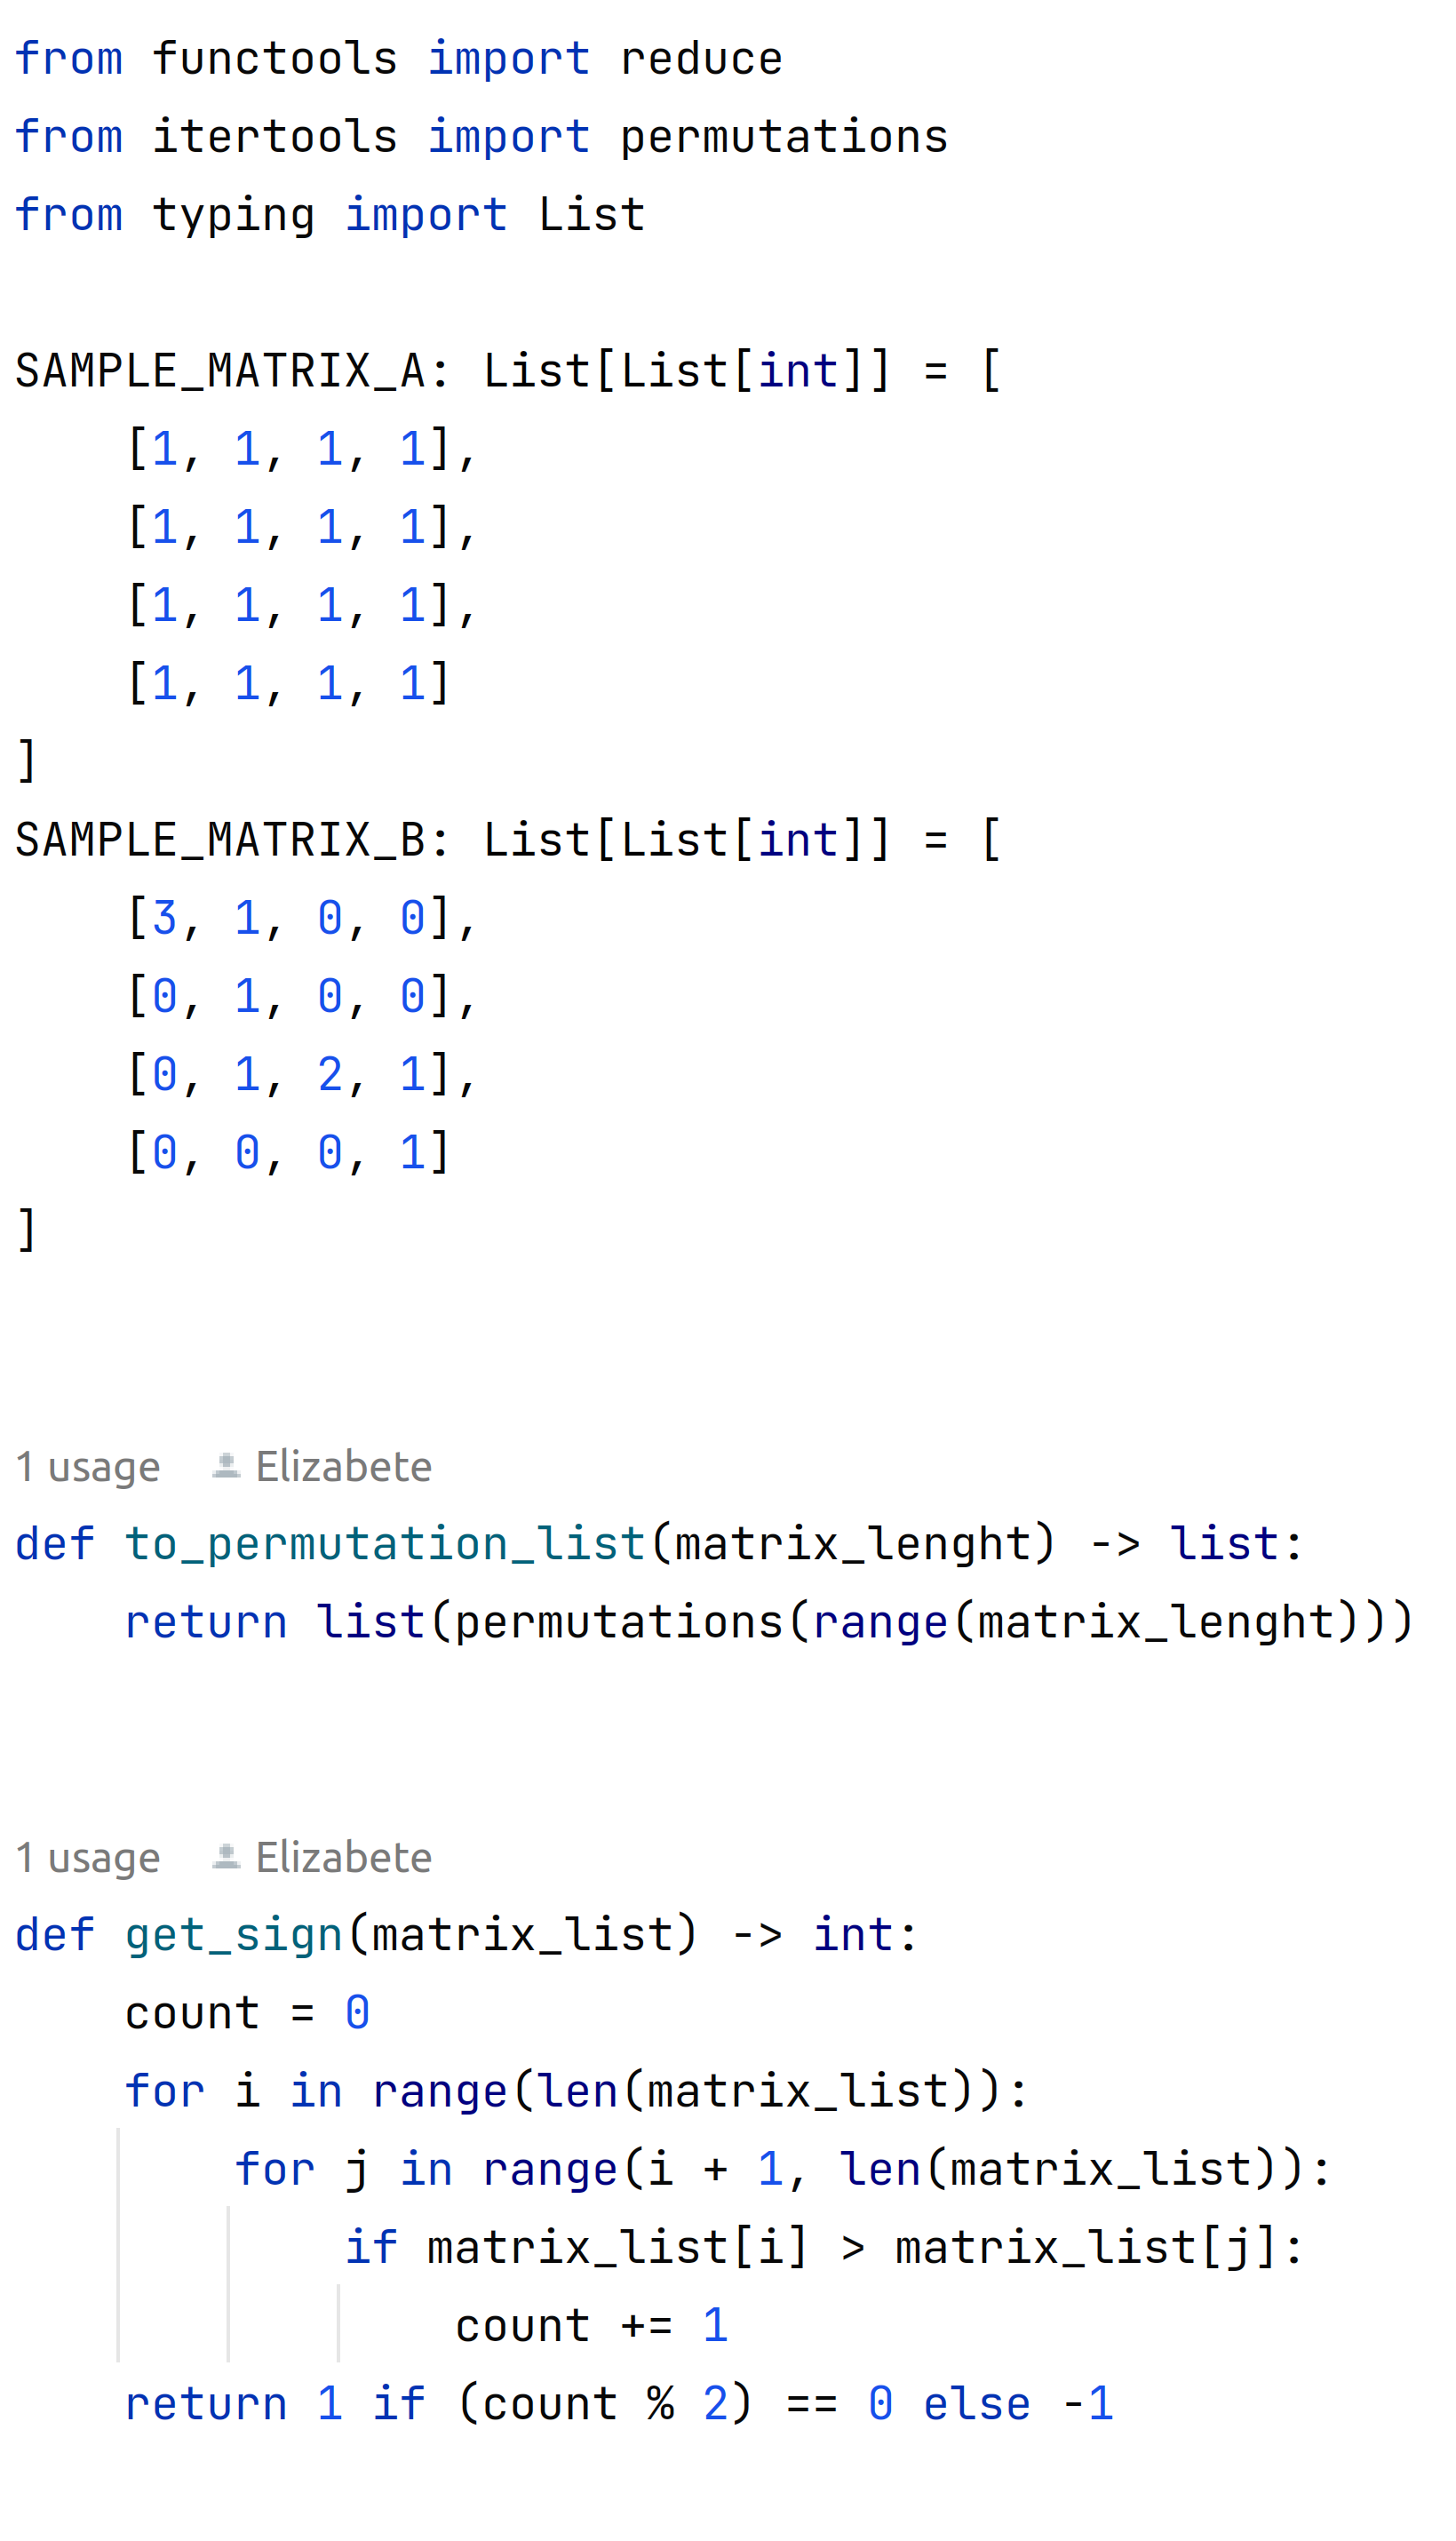
\includegraphics[width=10cm,]{code_01.png}
\caption{Parte 1}
\label{Rótulo}
\end{figure}

\begin{figure}[h!]
\centering
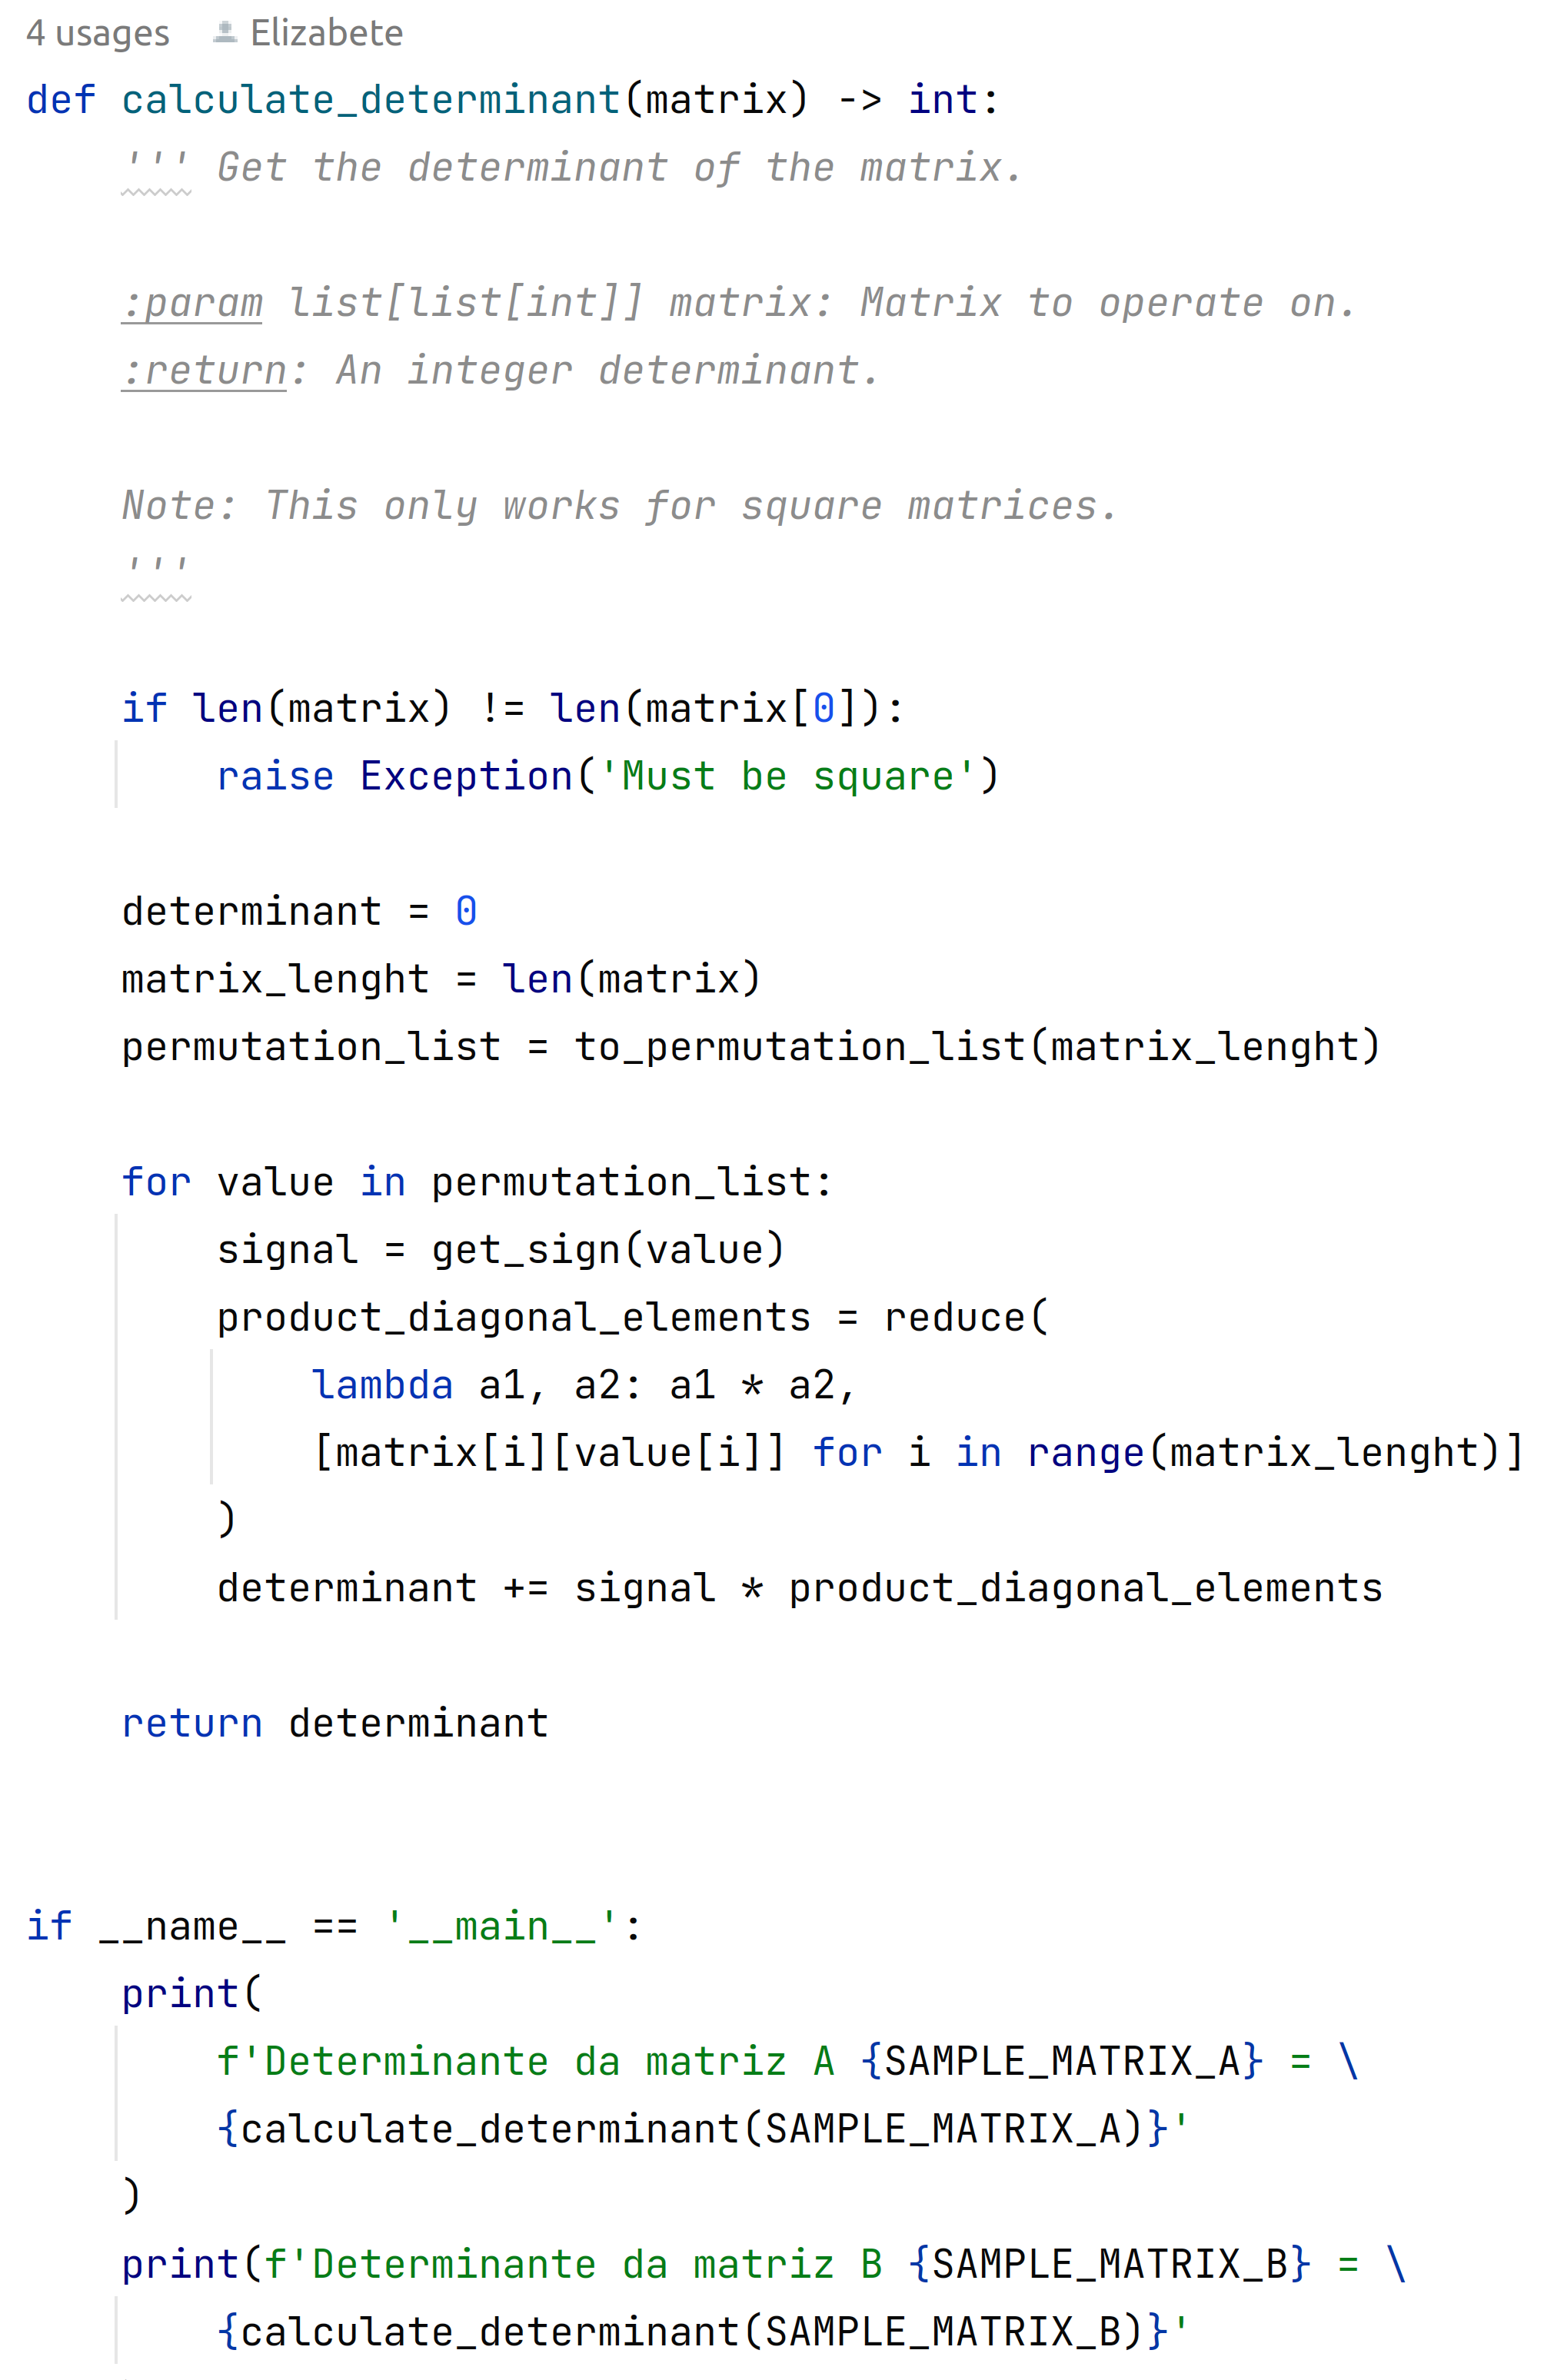
\includegraphics[width=12cm]{code_02.png}
\caption{Parte 2}
\label{Rótulo}
\end{figure}

\begin{figure}[h!]
\centering
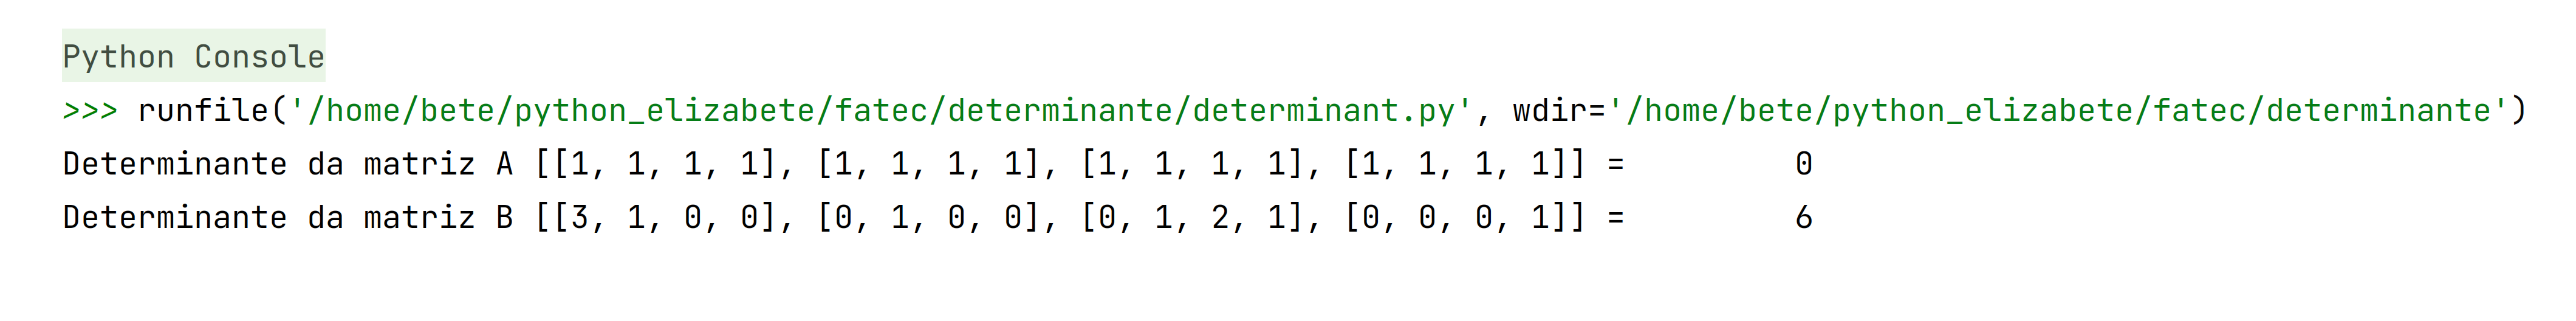
\includegraphics[width=18cm]{console.png}
\caption{Console}
\label{Rótulo}
\end{figure}

\end{document}

                                          